\section{Homepage}
In this section the homepage will be analyzed from the point of view of the usability. 
Since many components of the website are "shared" across different pages (they are the same even in internal pages), this section will contain also the analysis of the shared ones.

\subsection{Informative Axes}
The informative axes (6w) should provide the users with all the fundamental information regarding the website. 
If users are not able to collect those information, they are not willing to stay and navigate through the website, since they are not getting the information that they want.

\begin{figure}[h!]
	\centering
	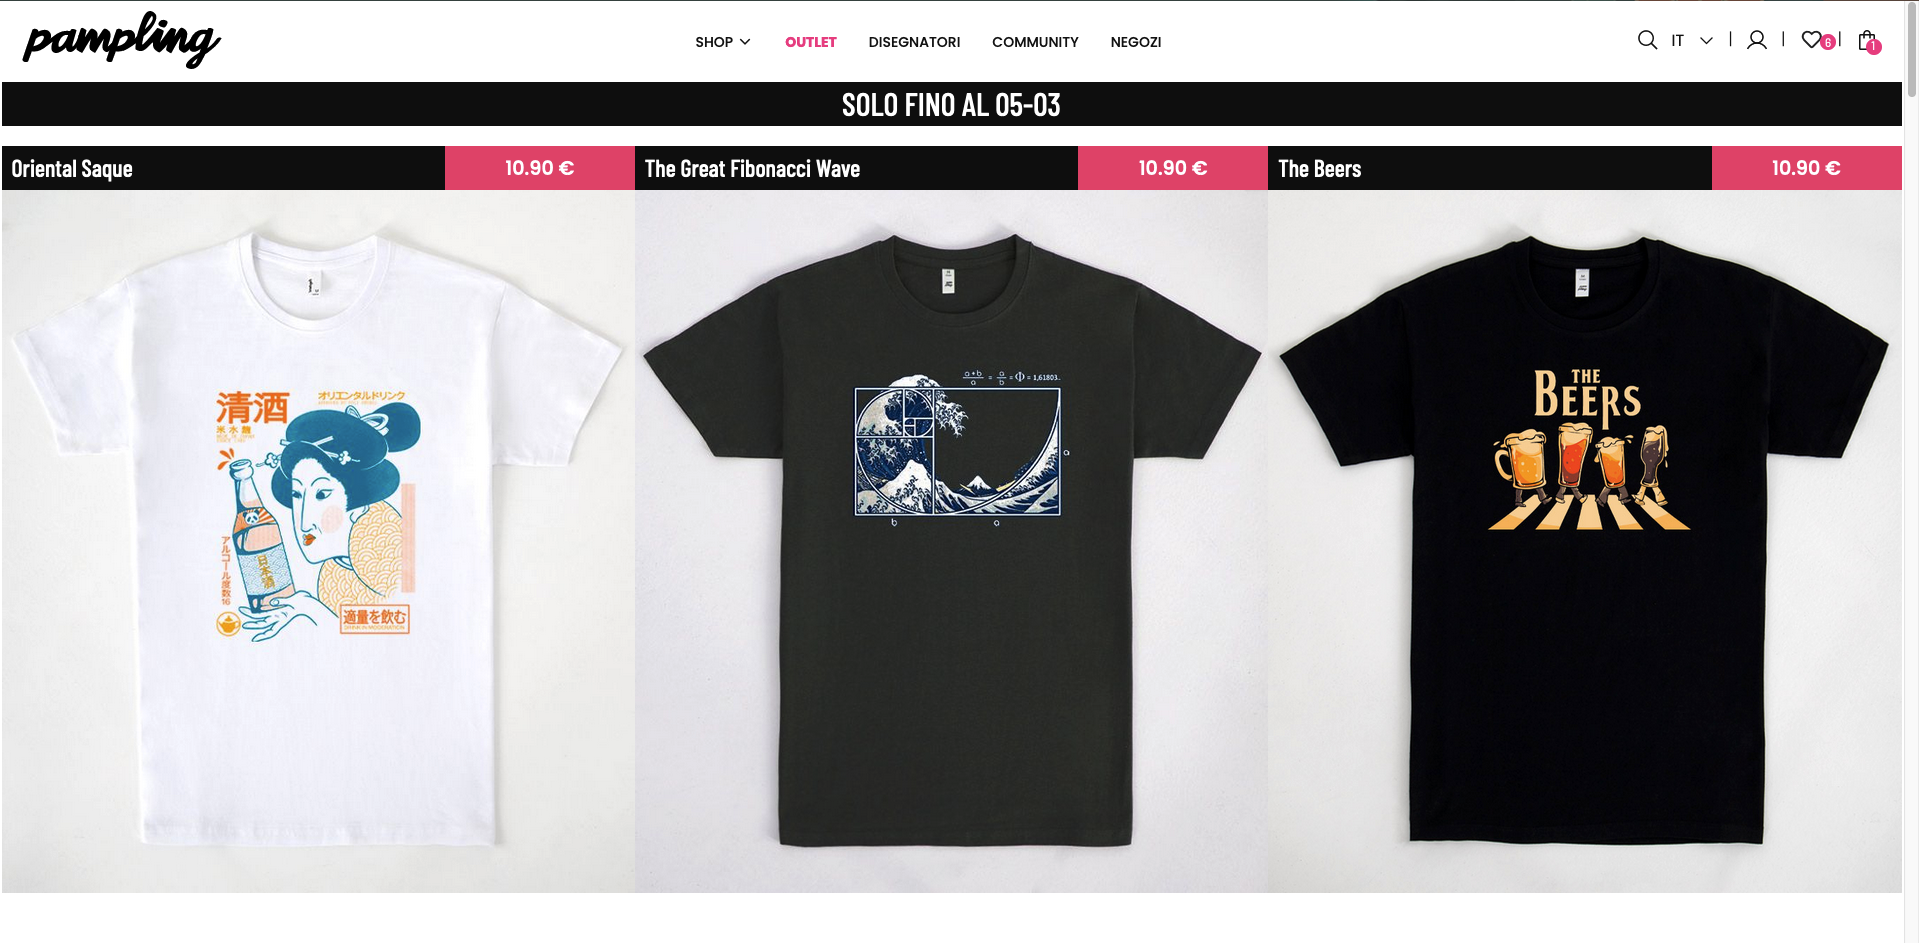
\includegraphics[scale=0.225]{images/homepage-first.png}
	\caption{homepage at first visit.}
	\label{fig:homepage-first}
\end{figure}

\subsubsection{WHERE did the user arrive?}
The website should give all the available information to the users regarding their relative position in the website, as well as a general idea about it. \\

If the where axis is not there, the user may experience the "lost in navigation" problem, which may lead to anger and frustration.\\
On the homepage of the website a complete menu of the website can be seen, that allows to reach all the possible pages of the website. 
On the top left corner of the homepage, in a standard position, there is the logo that links to the homepage.
The fact that the logo can be found in a standard position is a good choice, as the user will always be able to find it
and will be also able to find easily his way out of an unkown place.\\ 
Navigating through the website pages the breadcrumbs appear (of type "Location", which shows the absolute path from the website's root up to the specific page).
Not all the internal pages have them though, and this is not a good choice since it may lead to user confusion.

\subsubsection{WHO is behind the website?} 
The "who" axis should give the information about the website's owner.\\

Again, the logo in the top-left corner is really good to immediately understand the owner of the website. 
A good characteristic of the logo is that it is verbal and not just an image. 
A negative side is that the is no slogan of any kind: in this way, a user that arrives on the website without knowledge about this company
will not have many information about them.
In oder to get more information about the authors, the user is forced to scroll until the very end of the homepage. 
There he will find the footer (\cref{fig:footer}) where there may seem to be a link to a section of the website which aims to describe the company ("About Pampling").\\
Actually, if the user clicks there, the page shown is a FAQ page that does not give any information about the company.
Beacuse all of the points above, the "who" axis is not really satisfied and new users will have difficulties in understanding who's behind the site.

\begin{figure}[h!]
	\centering
	
\includegraphics[scale=0.225]{images/footer.png}
	\caption{footer of the website.}
	\label{fig:footer}
\end{figure}


\subsubsection{WHY should the user stay?} 
The "why" axis should provide motivations to users to persuade them to stay and navigate within the website.\\

The homepage without scrolling shows some offers currently active, that may catch the user attention and give a motivation to navigate further the website and that's positive.
On the other hand, the fact that these offers occupy the whole visible part of the homepage is not totally good, since it requires some scroll to the user to reach other content
that might be of better used if positioned at the start of the page.
  
Watching the homepage without scrolling would let the user unsatisfied concerning this informative axis. 
In fact there is no slogan or phrase that is capturing the user's attention. 
By scrolling (quite a bit), the user will see some sections containg \textit{catch phrases}. 
Examples in \cref{fig:slogan}.\\
The average user is not willing to scroll that much in the homepage, that is why putting \textit{catch content} that down (talking about scrolling) may not capture the users' attention.

\begin{figure}[h!]
	\centering
	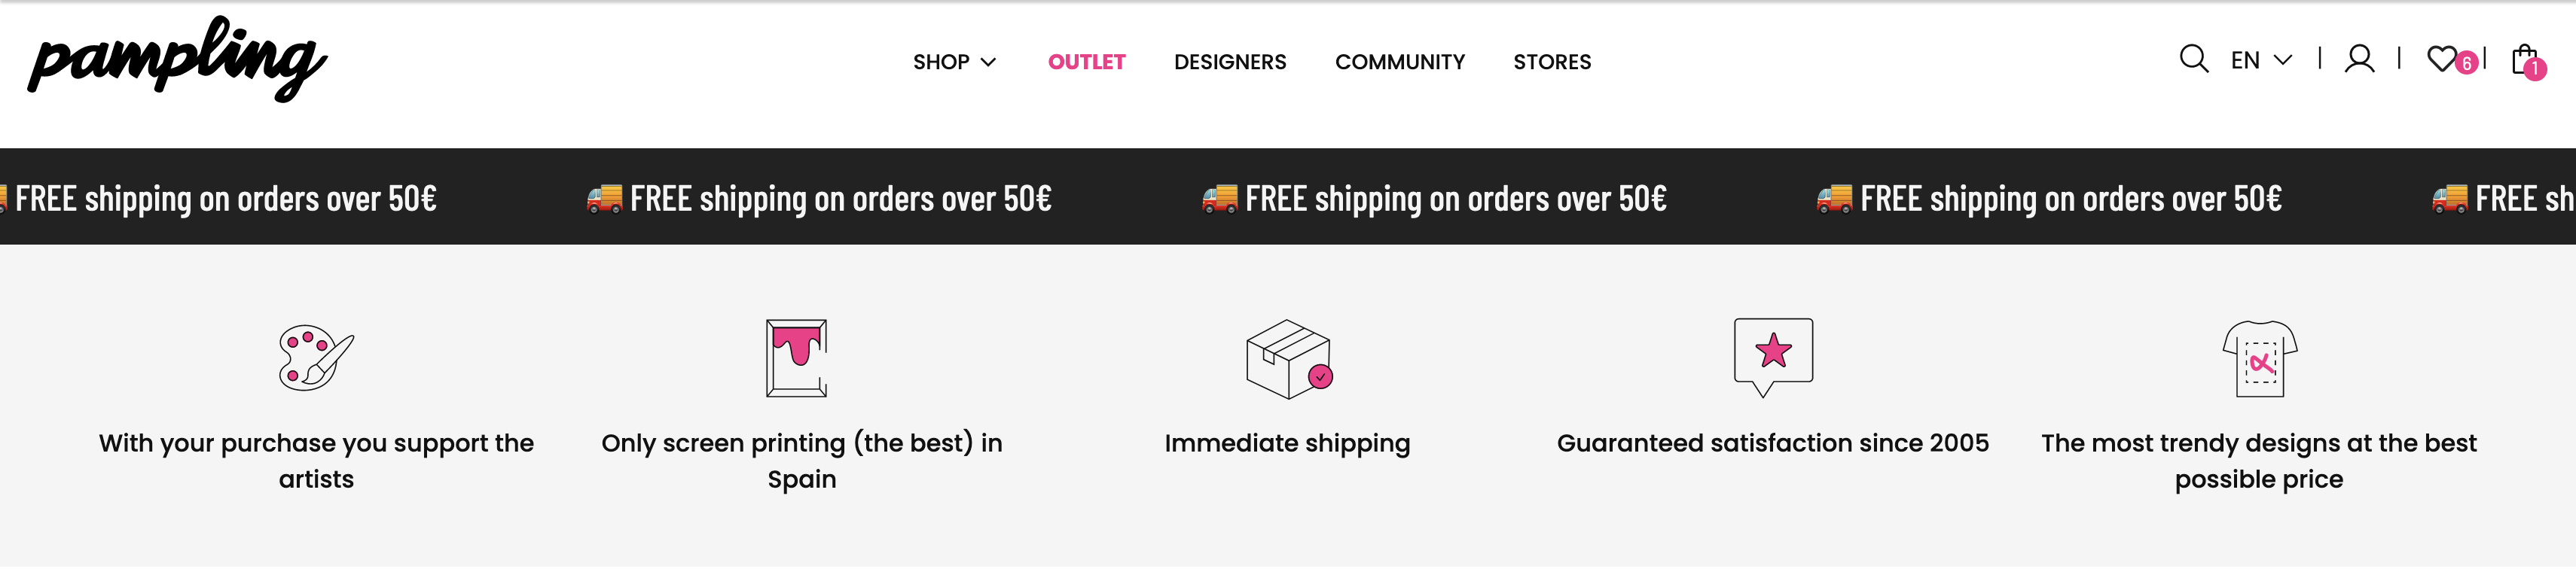
\includegraphics[scale=0.225]{images/slogan.png}
	\caption{slogans on the homepage.}
	\label{fig:slogan}
\end{figure}

\subsubsection{WHAT choices does the user have?} 
Another important axis is the "what" one. It should give the users access to all the possible destinations of the website.\\



\subsubsection{WHEN (latest news)} 
This axis should provide to the users all the latest news regarding the products and the company.\\


\subsubsection{HOW to arrive where the user wants?} 
The axis should offer tools to the users in order to let them access and collect information in a smart way.\\


\subsection{Asking for Personal Data}
The website is freely accessible by everyone. At the beginning of the visit there's no blocking pop-up asking for personal user data. So the website is not trying to collect users' data in order to create a kind of "club effect".\\
A random pop-up appears while scrolling the homepage the first time, as shown in \cref{fig:popup}. Since it is what it is (a popup), it is really annoying for the users. The only good thing about this negative situation, is that it can be easily removed and thus users are not required to fill it.


\subsection{Scrolling and Resolution}
\subsubsection{Scrolling}
Scrolling requires computational effort, that is why having too much scroll is bad. Typically users are willing to scroll up to 1.3 "screens" of a website page. Generally speaking, the quantity of scrolling may depend on the content of the page.\\

\paragraph{Vertical Scroll}

\paragraph{Horizontal Scroll}

\subsubsection{Resolution}
The homepage, and generally speaking the website, seems to not suffer of the "frozen layout" problem. In fact, even if the resolution changes, the web site is designed in such a way to fit the entire screen size (width) independently of the resolution. 


\subsection{Menu}
The homepage (and website) menu can be seen on \cref{fig:menu}. The menu is one of the most important components of a website: it allows the user to navigate through it and also to see what are the alternative information that can be found within the website.

The website's menu is a pretty common one. It is a horizontal menu with 6 entries. It has not a tree-like structure, since it is constructed on 2 informative levels only: the general one (first) and the detailed one (second, which shows all the options regarding a first-level entry).\\
The menu has been correctly implemented, since it avoids the \textit{horizontal menu - mouse} critical combo. In fact it has a max depth of 2 levels and for each entry a kind of subpage is offered to the user. In the subpage there are all the options related to the first-level entry. In such a way the user can comfortably choose the detailed option without performing many clicks. No fault-tolerance algorithm is required, since there is no possibility of having the menu to close when inside a first-level entry.\\
Overall the menu has been implemented in a really good way, by avoiding all the common and annying problems of the classic websites' menus.

\subsection{Content}
In this section the style of the main content of the homepage (and internal pages) will be analyzed. Since there is not much content in the homepage, the content analyzed will be the one of \cref{fig:content}.

\subsubsection{Text}
The text of the main content of the page must be readable. In order to achieve readability, a set of constraints must be respected.

\paragraph{Resizing Options}
There should be buttons (or even other ways) to allow the users to easily change the font size, without using zoom-in or zoom-out browser's tools.\\

The website is not offering resizing options at all. The only way to adjust the font size is by using the zoom functionality of the browser. Furthermore, there is an entry on the smaller menu (\cref{fig:menu}) called "Enable Accessibility" and even by clicking on it, nothing really happens.

\paragraph{Color and Font}
The font size is pretty big by default, surely bigger than 10 points (minimal one), which a strong advantage. In addition, only one font is used within all the website, which is, again, an optimal solutions.\\
Regarding text colors, nothing need to be said, as the main color is black on white background and white on dark background. That being said, even the contrast is pretty good, as the text is easily readable independently of the background.

\paragraph{Style}
The text is mainly in lowercase, which is really good since the user is not required to switch a lot between uppercase and lowercase while reading. There are just some phrases in uppercase, but they are detached from the main content and therefore they don't interfere with the user's reading.

\paragraph{Graphical Objects}
Finally, there is no text inside images (or graphical objects in general). That is another strong point, as text on images:
\begin{itemize}
\item Cannot be resized properly;
\item Will make the image to weight more, and thus more loading time;
\item Will make the "\textit{copy\&paste}" functionality to not work;
\item Will not be recognized by search engines that are crawling the webpage.
\end{itemize}

\subsubsection{Content Structure}
\paragraph{Structure}
Generally speaking, the content seems to not suffer of the "\textit{Lorem Ipsum}" problem (\textit{layout-design-first} problem). In fact the content looks like to be well structured, therefore the initial scanning phase is likely to be successful.\\
Each paragraph is not too big, and it is always preceded by a descriptive title. That is another advantage of the website, as the users' understanding process is helped and so it will be easier. Since paragraphs are not too long, maybe it is not strictly necessary to put blurbs (summaries), even if users would appreciate them anyway.

\paragraph{Keywords}

\paragraph{Lists}

\paragraph{Column}

\subsection{Attention Map}

\subsubsection{F-shape Map}
The \textit{F-shape} map of attention states that the most important components of the webpage should be placed within the center of the webpage, keeping in mind that being on the top of the page is better rather than being on the bottom.\\

\subsubsection{Images}

\subsection{Searching}
Without knowing the exact number of pages of the website, it looks not too big, certainly below the 100 pages treshold. It means that the search functionality is not strictly required, as having a good navigation system may be more than enough.\\
If the search tool is available, users will certainly use it, as in the case of this website.

\subsubsection{Search Tools}
The search functionality can be activated by clicking on the lens icon, placed near the top-right corner.


\subparagraph{No Result}
\begin{figure}[h!]
	\centering
	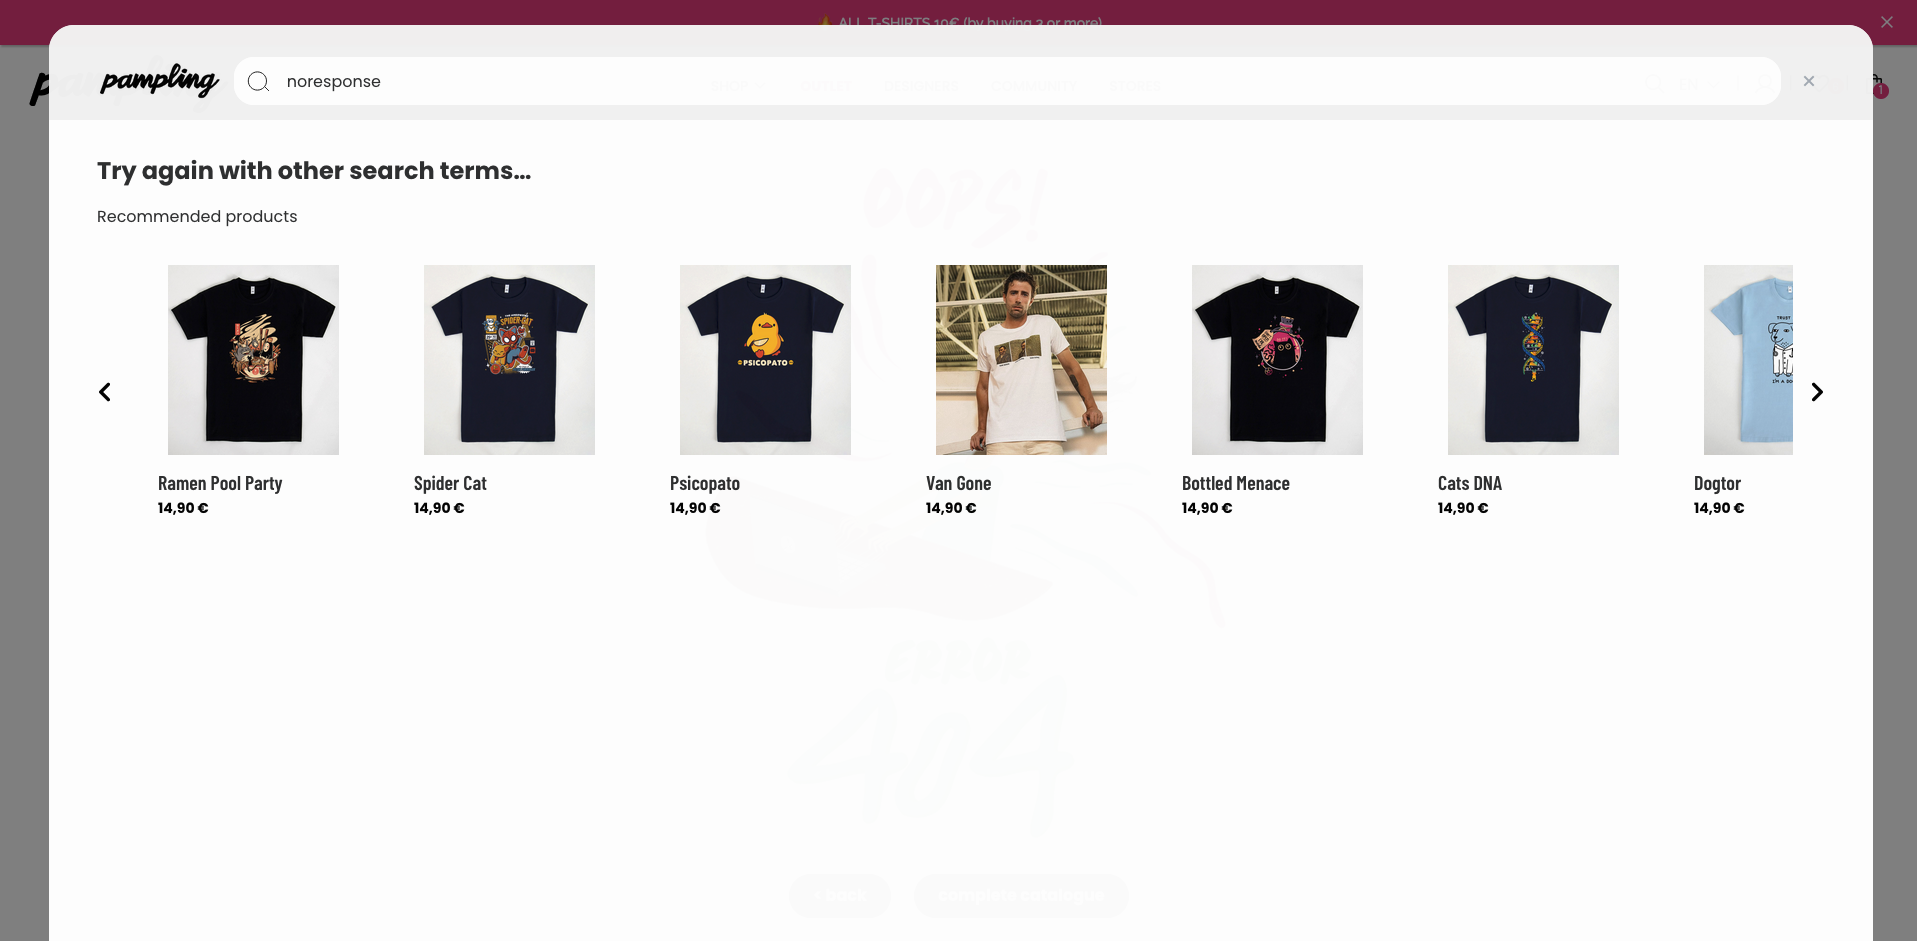
\includegraphics[scale=0.225]{images/zero-res.png}
	\caption{no result webpage.}
	\label{fig:zero-res}
\end{figure}

In \cref{fig:zero-res}, it is possible to see how the website handles no results for a certain keyword. How the website handles this particular situation is not really good.\\
First of all, it is not trying to recover from errors: putting a single typo within a known keyword ("camere" instead of "camera") will cause the search to fail. Maybe it would have been better to implement some kind of fault tolerance on the text inserted within the searchbox.\\
The webpage then shows a list of related pages (big buttons), that may help the user to find himself out of nowhere, which is good.

\subparagraph{404 Page}
\begin{figure}[h!]
	\centering
	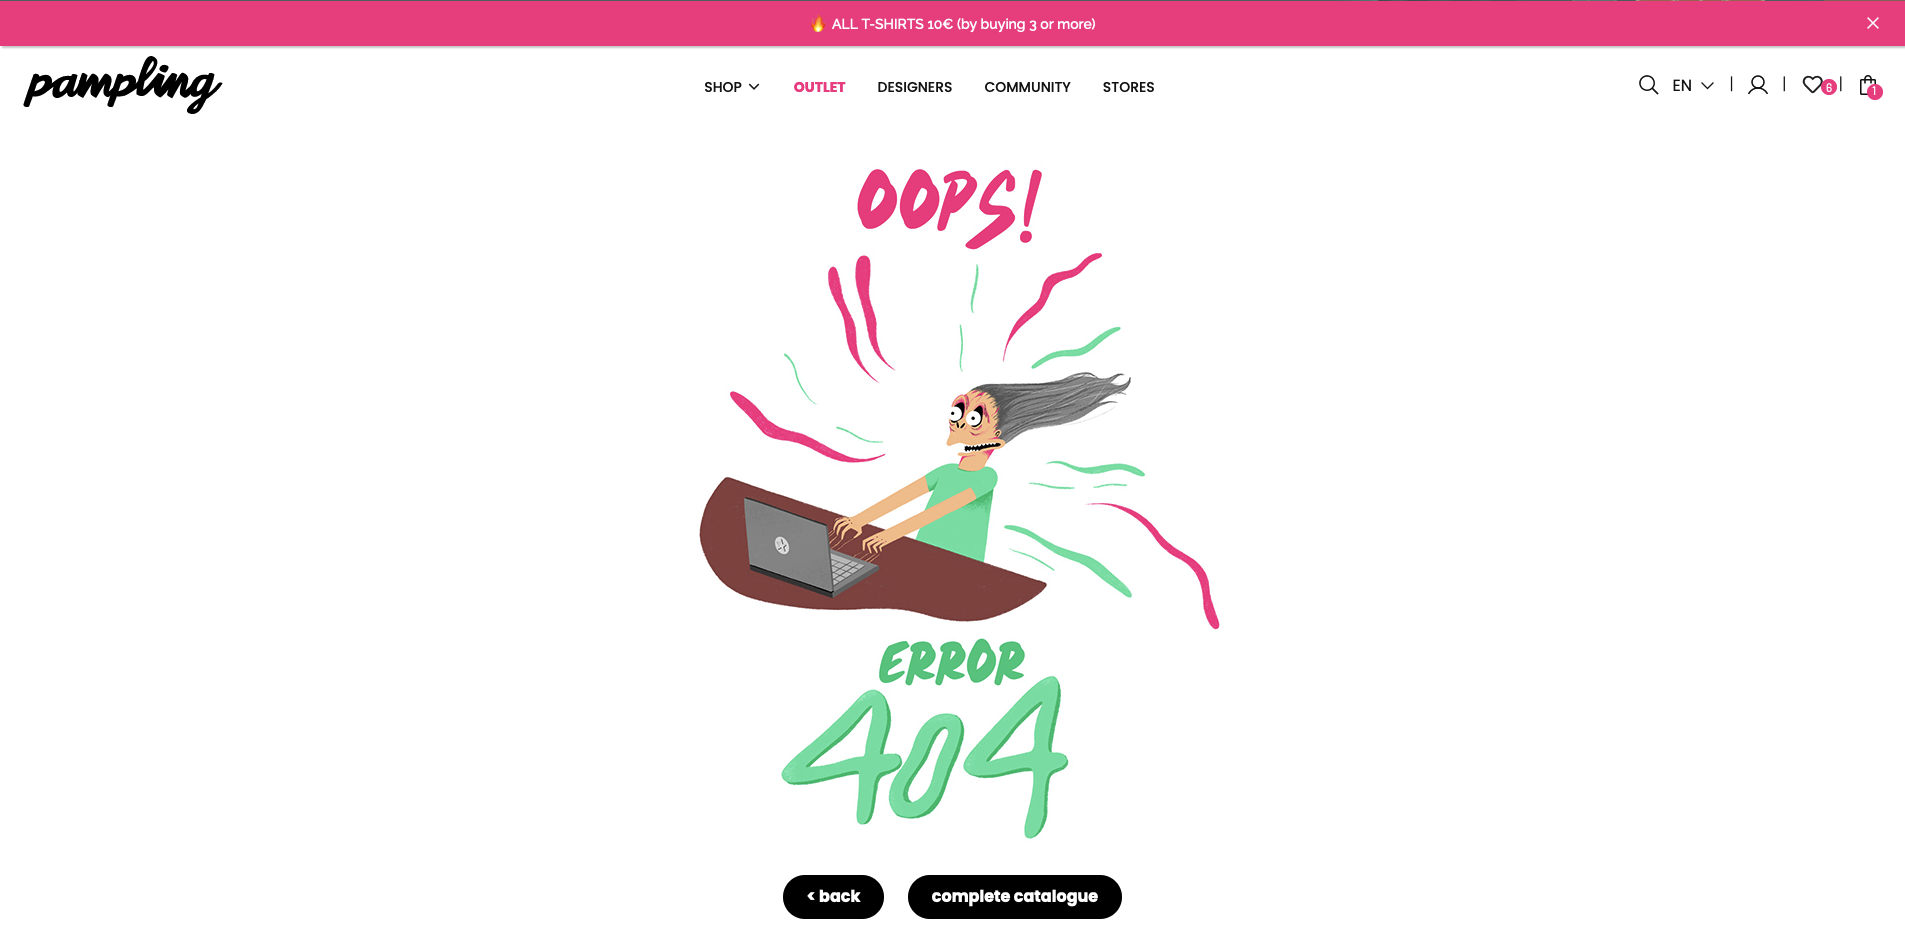
\includegraphics[scale=0.225]{images/404.png}
	\caption{404 webpage.}
	\label{fig:404}
\end{figure}

A 404 HTTP error occurs when the webpage required is not available or it does not exist anymore. Since, once again, it can happen, it is important to handle even the case of broken links or typos in URLs.\\
The website's 404 page is pretty well designed. Firstly, it is offering a full menu (the classic one) as well as the search tool.\\
It is not mentioning technical aspects such as "404 error", "wrong URL" and so on: that is really good, as users are being confused by reading terms that they may never heard about.\\
The page is also make a kind of a joke, in such a way it tries to turn a bad situation into a positive one with a simple but effective metaphor.\\
Lastly, the page is offering references (links) to the most popular pages of the website, so the user is not required to go deep into the menu at first.\\
Overall, the user experience, even with a 404 error, is pretty good.

\paragraph{Search Result Presentation}
The output of a search cannot really be seen, since every time a search is performed, the result will be either the webpage that matches the best the query or the "No result" webpage.\\
There is no grid presentation of the results and so on.

\subsubsection{Search Box}
The length of users' queries increased a lot in past years, as a result of having much more information available on the web. It is important to offer a textual box which is sufficiently large, in order to not force the users to write shorter queries (and thus having less precise results).\\

The search tool offered by the website can be activated by clicking on the lens icon. Once clicked, a big search box will appear. It is the biggest one available, since it is covering the entire width of the layout. That is great, as the user will fell comfortable and the website will not pay time penalties as a result of small search boxes.